\documentclass{standalone}
\usepackage{pgfplots}
\pgfplotsset{soldot/.style={color=black,only marks,mark=*},
             holdot/.style={color=black,fill=white,only marks,mark=*},
             compat=1.12}
\begin{document}
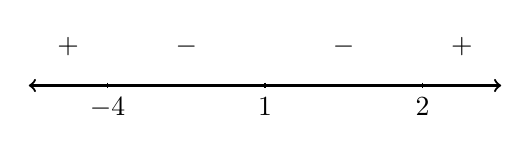
\begin{tikzpicture}
\draw[thick,<->] (-.5,0) -- (5.5,0);
 \draw (.5 cm,1pt) -- (.5 cm,-1pt) node[anchor=north] {$-4$};
  \draw (2.5 cm,1pt) -- (2.5 cm,-1pt) node[anchor=north] {$1$};
   \draw (4.5 cm,1pt) -- (4.5 cm,-1pt) node[anchor=north] {$2$};
 \draw (0,.5) node {+};
 \draw (1.5,.5) node {$-$};
  \draw (3.5,.5) node {$-$};
    \draw (5,.5) node {$+$};
\end{tikzpicture}
\end{document}